%%%%%%%%%%%%%%%%%%%%%%%%%%%%%%%%%%%%%%%%%
% Beamer Presentation
% LaTeX Template
% Version 1.0 (10/11/12)
%
% This template has been downloaded from:
% http://www.LaTeXTemplates.com
%
% License:
% CC BY-NC-SA 3.0 (http://creativecommons.org/licenses/by-nc-sa/3.0/)
%
%%%%%%%%%%%%%%%%%%%%%%%%%%%%%%%%%%%%%%%%%

%----------------------------------------------------------------------------------------
%	PACKAGES AND THEMES
%----------------------------------------------------------------------------------------

\documentclass{beamer}

\mode<presentation> {

% The Beamer class comes with a number of default slide themes
% which change the colors and layouts of slides. Below this is a list
% of all the themes, uncomment each in turn to see what they look like.

%\usetheme{default}
%\usetheme{AnnArbor}
%\usetheme{Antibes}
%\usetheme{Bergen}
%\usetheme{Berkeley}
%\usetheme{Berlin}
%\usetheme{Boadilla}
%\usetheme{CambridgeUS}
%\usetheme{Copenhagen}
%\usetheme{Darmstadt}
%\usetheme{Dresden}
%\usetheme{Frankfurt}
%\usetheme{Goettingen}
%\usetheme{Hannover}
%\usetheme{Ilmenau}
%\usetheme{JuanLesPins}
%\usetheme{Luebeck}
\usetheme{Madrid}
%\usetheme{Malmoe}
%\usetheme{Marburg}
%\usetheme{Montpellier}
%\usetheme{PaloAlto}
%\usetheme{Pittsburgh}
%\usetheme{Rochester}
%\usetheme{Singapore}
%\usetheme{Szeged}
%\usetheme{Warsaw}

% As well as themes, the Beamer class has a number of color themes
% for any slide theme. Uncomment each of these in turn to see how it
% changes the colors of your current slide theme.

%\usecolortheme{albatross}
%\usecolortheme{beaver}
%\usecolortheme{beetle}
%\usecolortheme{crane}
%\usecolortheme{dolphin}
%\usecolortheme{dove}
%\usecolortheme{fly}
%\usecolortheme{lily}
%\usecolortheme{orchid}
%\usecolortheme{rose}
%\usecolortheme{seagull}
%\usecolortheme{seahorse}
%\usecolortheme{whale}
%\usecolortheme{wolverine}

%\setbeamertemplate{footline} % To remove the footer line in all slides uncomment this line
%\setbeamertemplate{footline}[page number] % To replace the footer line in all slides with a simple slide count uncomment this line

%\setbeamertemplate{navigation symbols}{} % To remove the navigation symbols from the bottom of all slides uncomment this line
}

\usepackage{geometry}
\usepackage{multimedia}  % Allows including videos
\usepackage{graphicx}    % Allows including images
\usepackage{bm}          % Allows nice bold math
\usepackage{color}       % Allows color
\usepackage{array,booktabs,calc} % Allows nice multi-figure layout
\usepackage{setspace}

\definecolor{light_green}{rgb}{0.8,1.,0.8}
\definecolor{light_yellow}{rgb}{1.,1.,0.8}
\definecolor{yellow}{rgb}{1.,1.,0.}
\definecolor{orange}{rgb}{0.9,0.4,0.}
\definecolor{pink}{rgb}{1.,0.6,1.}
\definecolor{dark_green}{rgb}{0.1,0.6,0.1}
\definecolor{light_blue}{rgb}{0.6,0.6,1.}
\definecolor{purple}{rgb}{0.8,0.0,0.8}
\def\oran#1{\color{orange} #1}
\def\gr#1{\color{dark_green} #1}
\def\re#1{\color{red}   #1}
\def\bl#1{\color{blue}  #1}
\def\pu#1{\color{purple} #1}
\def\bk#1{\color{black} #1}
\def\lb#1{\color{light_blue} #1}
\def\pk#1{\color{pink} #1}
\def\ye#1{\color{yellow} #1}

\providecommand\der{{\rm d}}
\providecommand\Der{{\rm D}}
\providecommand\pa{{\partial}}
\def\pp#1#2{\frac{\pa  #1}{\pa  #2}}
\def\dd#1#2{\frac{\der #1}{\der #2}}
\def\DD#1#2{\frac{\Der #1}{\Der #2}}

\def\ltw{{\hbox{${\lower 6pt\hbox{$<$}}\atop{\raise 2pt\hbox{$\sim$}}$}\,}}
\def\gtw{{\hbox{${\lower 6pt\hbox{$>$}}\atop{\raise 2pt\hbox{$\sim$}}$}\,}}

\newcommand\shalf{\ensuremath{{\scriptstyle\frac{1}{2}}}}
\newcommand\sh{\ensuremath{^{\shalf}}}
\newcommand\sthalf{\ensuremath{{\scriptstyle\frac{3}{2}}}}
\newcommand\sth{\ensuremath{^{\sthalf}}}
\newcommand\smh{\ensuremath{^{-\shalf}}}
\newcommand\squart{\ensuremath{{\textstyle\frac{1}{4}}}}
\newcommand\thalf{\ensuremath{{\textstyle\frac{1}{2}}}}

\newcommand{\cO}{\ensuremath{\mathcal{O}}}
\newcommand{\cC}{\ensuremath{\mathcal{C}}}
\newcommand{\cD}{\ensuremath{\mathcal{D}}}
\newcommand{\cF}{\ensuremath{\mathcal{F}}}

\newcommand{\bel}{\ensuremath{b_\ell}}
\newcommand{\bli}{\ensuremath{b_{\ell i}}}
\newcommand{\blb}{\ensuremath{b_{\ell 0}}}
\newcommand{\thlo}{\ensuremath{\theta_{\ell 0}}}
\newcommand{\thpl}{\ensuremath{\theta'_{\ell}}}

\newsavebox{\AAbox} \sbox{\AAbox}{\boldmath$A$}
\newcommand{\Abf}{\usebox{\AAbox}}

\newsavebox{\SSbox} \sbox{\SSbox}{\boldmath$S$}
\newcommand{\Sbf}{\usebox{\SSbox}}

\newsavebox{\FFbox} \sbox{\FFbox}{\boldmath$F$}
\newcommand{\Fbf}{\usebox{\FFbox}}

\newsavebox{\GGbox} \sbox{\GGbox}{\boldmath$G$}
\newcommand{\Gbf}{\usebox{\GGbox}}

\newsavebox{\HHbox} \sbox{\HHbox}{\boldmath$H$}
\newcommand{\Hbf}{\usebox{\HHbox}}

\newsavebox{\eebox} \sbox{\eebox}{\boldmath$e$}
\newcommand{\ee}{\usebox{\eebox}}
\newcommand{\eex}{\ensuremath{\hat{\ee}_x}}
\newcommand{\eey}{\ensuremath{\hat{\ee}_y}}
\newcommand{\eez}{\ensuremath{\hat{\ee}_z}}

\newcommand{\bcdot}{\bm \cdot}
\newcommand{\oo}{\bm \omega}
\newcommand{\uu}{\bm u}
\newcommand{\xx}{\bm x}
\newcommand{\XX}{\bm X}

\newcommand{\grad}{\bm \nabla}
\newcommand{\degrees}{\mbox{$^{\circ}$}}

\let\vaccent=\v % rename builtin command \v{} to \vaccent{}
\renewcommand{\v}[1]{\ensuremath{\mathbf{#1}}} % for vectors
%\renewcommand{\v}[1]{\ensuremath{\mbox{\boldmath$ #1 $}}}
\newcommand{\gv}[1]{\ensuremath{\mbox{\boldmath$ #1 $}}}
% for vectors of Greek letters
\newcommand{\uv}[1]{\hat{\ensuremath{\mathbf{ #1 }}}} % for unit vector
\newcommand{\abs}[1]{\left| #1 \right|} % for absolute value
\newcommand{\avg}[1]{\left< #1 \right>} % for average
\let\underdot=\d % rename builtin command \d{} to \underdot{}
\renewcommand{\d}[2]{\frac{d #1}{d #2}} % for derivatives
\newcommand{\pd}[2]{\frac{\partial #1}{\partial #2}}
% for partial derivatives
\let\divsymb=\div % rename builtin command \div to \divsymb
\renewcommand{\div}[1]{\v{\nabla} \cdot #1} % for divergence
\newcommand{\curl}[1]{\v{\nabla} \times #1} % for curl

\usepackage{fancyvrb}
\DefineShortVerb[commandchars=\\\{\}]{\|}
\DefineVerbatimEnvironment{Highlighting}{Verbatim}{commandchars=\\\{\}}
% Add ',fontsize=\small' for more characters per line
\newenvironment{Shaded}{}{}
\newcommand{\KeywordTok}[1]{\textcolor[rgb]{0.13,0.29,0.53}{\textbf{{#1}}}}
\newcommand{\DataTypeTok}[1]{\textcolor[rgb]{0.13,0.29,0.53}{{#1}}}
\newcommand{\DecValTok}[1]{\textcolor[rgb]{0.00,0.00,0.81}{{#1}}}
\newcommand{\BaseNTok}[1]{\textcolor[rgb]{0.00,0.00,0.81}{{#1}}}
\newcommand{\FloatTok}[1]{\textcolor[rgb]{0.00,0.00,0.81}{{#1}}}
\newcommand{\ConstantTok}[1]{\textcolor[rgb]{0.00,0.00,0.00}{{#1}}}
\newcommand{\CharTok}[1]{\textcolor[rgb]{0.31,0.60,0.02}{{#1}}}
\newcommand{\SpecialCharTok}[1]{\textcolor[rgb]{0.00,0.00,0.00}{{#1}}}
\newcommand{\StringTok}[1]{\textcolor[rgb]{0.31,0.60,0.02}{{#1}}}
\newcommand{\VerbatimStringTok}[1]{\textcolor[rgb]{0.31,0.60,0.02}{{#1}}}
\newcommand{\SpecialStringTok}[1]{\textcolor[rgb]{0.31,0.60,0.02}{{#1}}}
\newcommand{\ImportTok}[1]{{#1}}
\newcommand{\CommentTok}[1]{\textcolor[rgb]{0.56,0.35,0.01}{\textit{{#1}}}}
\newcommand{\DocumentationTok}[1]{\textcolor[rgb]{0.56,0.35,0.01}{\textbf{\textit{{#1}}}}}
\newcommand{\AnnotationTok}[1]{\textcolor[rgb]{0.56,0.35,0.01}{\textbf{\textit{{#1}}}}}
\newcommand{\CommentVarTok}[1]{\textcolor[rgb]{0.56,0.35,0.01}{\textbf{\textit{{#1}}}}}
\newcommand{\OtherTok}[1]{\textcolor[rgb]{0.56,0.35,0.01}{{#1}}}
\newcommand{\FunctionTok}[1]{\textcolor[rgb]{0.00,0.00,0.00}{{#1}}}
\newcommand{\VariableTok}[1]{\textcolor[rgb]{0.00,0.00,0.00}{{#1}}}
\newcommand{\ControlFlowTok}[1]{\textcolor[rgb]{0.13,0.29,0.53}{\textbf{{#1}}}}
\newcommand{\OperatorTok}[1]{\textcolor[rgb]{0.81,0.36,0.00}{\textbf{{#1}}}}
\newcommand{\BuiltInTok}[1]{{#1}}
\newcommand{\ExtensionTok}[1]{{#1}}
\newcommand{\PreprocessorTok}[1]{\textcolor[rgb]{0.56,0.35,0.01}{\textit{{#1}}}}
\newcommand{\AttributeTok}[1]{\textcolor[rgb]{0.77,0.63,0.00}{{#1}}}
\newcommand{\RegionMarkerTok}[1]{{#1}}
\newcommand{\InformationTok}[1]{\textcolor[rgb]{0.56,0.35,0.01}{\textbf{\textit{{#1}}}}}
\newcommand{\WarningTok}[1]{\textcolor[rgb]{0.56,0.35,0.01}{\textbf{\textit{{#1}}}}}
\newcommand{\AlertTok}[1]{\textcolor[rgb]{0.94,0.16,0.16}{{#1}}}
\newcommand{\ErrorTok}[1]{\textcolor[rgb]{0.64,0.00,0.00}{\textbf{{#1}}}}
\newcommand{\NormalTok}[1]{{#1}}
%~ \ifxetex
  %~ \usepackage[setpagesize=false, % page size defined by xetex
              %~ unicode=false, % unicode breaks when used with xetex
              %~ xetex,
              %~ colorlinks=true,
              %~ linkcolor=blue]{hyperref}
%~ \else
  %~ \usepackage[unicode=true,
              %~ colorlinks=true,
              %~ linkcolor=blue]{hyperref}
%~ \fi
\hypersetup{breaklinks=true, pdfborder={0 0 0}}
\setlength{\parindent}{0pt}
\setlength{\parskip}{6pt plus 2pt minus 1pt}
\setlength{\emergencystretch}{3em}  % prevent overfull lines
\setcounter{secnumdepth}{0}

%\EndDefineVerbatimEnvironment{Highlighting}

\newcolumntype{C}[1]{>{\centering\arraybackslash}m{#1}}
\providecommand{\tightlist}{%
  \setlength{\itemsep}{0pt}\setlength{\parskip}{0pt}}

%----------------------------------------------------------------------------------------
%	TITLE PAGE
%----------------------------------------------------------------------------------------
%\title[LES discussions]{LES and more...}

\title[MPIC]{Webinar: Parallel Moist Parcel-In-Cell code}

\author[B\"oing, Gibb, Dritschel, et al.]{{Steef B\"oing, Gordon Gibb, David Dritschel, Nick Brown, \newline Mich\`ele Weiland, Doug Parker \& Alan Blyth}\vspace{-0.5cm}}

\institute[]{{University of Leeds, University of St Andrews, EPCC}\vspace{-0.4cm}}

\date{November 13, 2019}

\begin{document}

\begin{frame}

\titlepage % Print the title page as the first slide

\vspace{-0.6cm}
\begin{center}
%  \includegraphics[width = \textwidth]{pmpic_images/vorpic-cropped.pdf}
  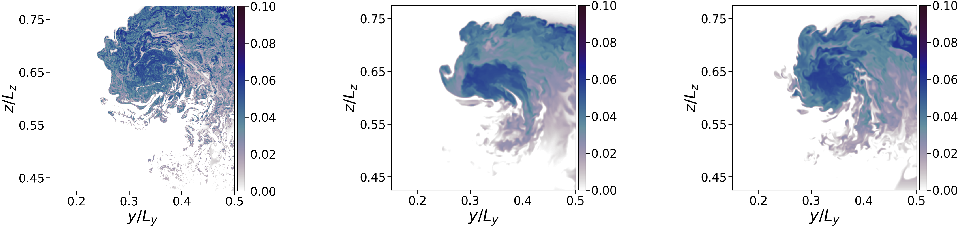
\includegraphics[width = \textwidth]{pmpic_images/croppedfig_les.pdf}
\end{center}

\setstretch{0.3} 

\end{frame}

\begin{frame}

\tableofcontents
\end{frame}

\begin{frame}
\frametitle{eCSE project 12-10}
\textit{A fully Lagrangian dynamical core for the Met Office NERC Cloud Model}
\vspace{-0.2cm}
\begin{center}
St Andrews, Leeds, EPCC
\end{center}
\vspace{-0.2cm}
\begin{itemize}
\item Most fluid dynamics codes are either fully Eulerian (grid-based), or semi-Lagrangian (advection using \textit{departure points} and regridding)
\item Here: \textit{essentially Lagrangian} (prognostics on parcels, solver uses grid)
\item Atmospheric Large-Eddy Simulation: e.g. Met Office/NERC Cloud model (MONC). 
\item Evaporation and condensation in clouds: discontinuity in underlying equations.
\end{itemize}
\vspace{-0.8cm}

\begin{center}
  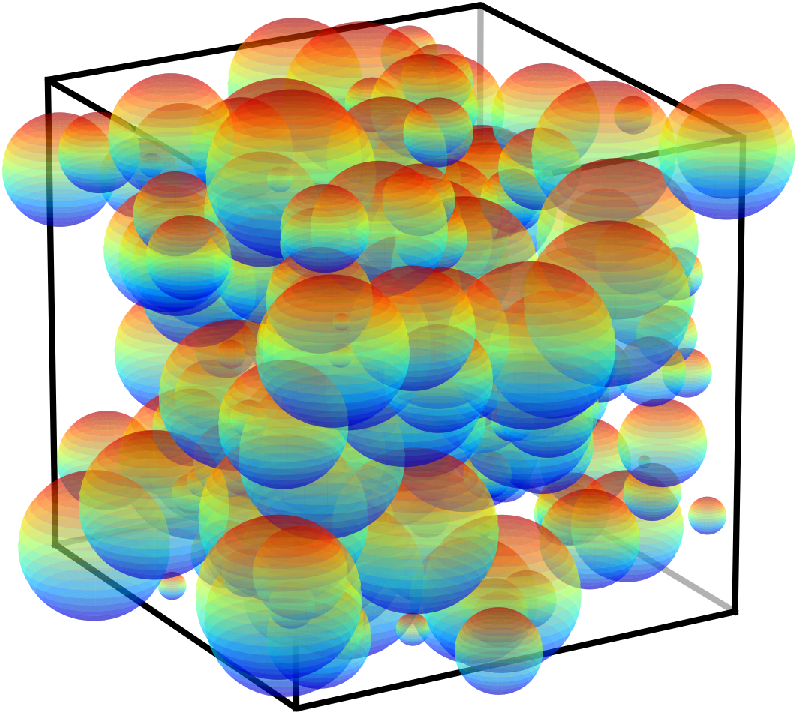
\includegraphics[width = 0.28\textwidth]{pmpic_images/parcels.pdf}
\end{center}

\end{frame}

\section{Moist Parcel-in-Cell code: overview}

%------------------------------------------------
\begin{frame}
\frametitle{Essentially Lagrangian modelling}

\begin{block}{}
{\bl The basic conservation principles} of fluid dynamics 
{\gr are naturally expressed} in a {\pu Lagrangian} way: 
e.g.\ mass is conserved {\it \re following} fluid ``parcels''.
\end{block}

\vspace{0.5cm}
{\re However}, certain fields are more naturally Eulerian in character,
e.g.\ pressure.  Here, one needs to solve for the entire field through
``inversion''.

\vspace{0.3cm}
\begin{block}{}
{\gr Conservation is Lagrangian.}  {\pu Inversion is Eulerian.}  
\end{block}

\vspace{0.5cm}
{\it Can we exploit this for simulation?}

\end{frame}

%-------------------------------------------------------------------

\begin{frame}
\frametitle{Moist Parcel-In-Cell (MPIC)}

The new ``Moist Parcel-In-Cell'' (MPIC) algorithm 
{\re represents the continuum by discrete} {\bl ``cloud (or environment) parcels''}.

\vspace{0.15cm}
We use {\pu freely-moving} 
{\pu parcels} carrying {\it any number} of {\re attributes} 
(e.g.\ {\bl a conserved temperature} 
$b_\ell$, {\bl specific humidity} $q$, etc...)

\vspace{0.15cm}
Prototype model for 3D incompressible flow
(Boussinesq, no rotation, no precipitation, non-dimensional):
\begin{flalign}
\DD{\uu}{t} & = - \frac{\grad{p}}{\rho_0} + b \uv{z} \qquad & \textsf{momentum} \nonumber \\ 
\DD{\bel}{t}&  = 0  \qquad & \textsf{conserved temperature} \nonumber \\
\DD{q}{t} & = 0  \qquad & \textsf{specific humidity, total amount of water} \nonumber \\
\grad\bcdot\uu & =0  \qquad & \textsf{incompressibility} \nonumber  \\
\nonumber
\end{flalign}

\end{frame}

\begin{frame}
\frametitle{Phase transitions}
The {\re total buoyancy} $b$ is approximated by
\begin{flalign}
b & = \bel+\alpha q_\ell \nonumber \\
q_\ell & =q-q_s(z) \textsf{ if } q>q_s(z) \textsf{, otherwise 0}.
\nonumber
\end{flalign}

$q_\ell$ is the {\bl liquid water content}. \newline
$q_s$ is the {\oran saturation humidity}, which decreases with height. \newline
$\alpha$ is a scale factor related to the {\re latent heat of condensation.} \newline

\end{frame}

\begin{frame}
\frametitle{Numerical implementation}

We evolve vorticity (instead of momentum) and parcel position using RK4

\begin{equation}
  \DD{\gv{\omega}}{t} = ( \div{\v{F}},\div{\v{G}},\div{\v{H}}), \nonumber
\end{equation}
Where $\v{F} = \gv{\omega}u + b \uv{y} $, $\v{G}=\gv{\omega}v - b \uv{x}$, $\v{H}=\gv{\omega}w$ and $\v{u}= (u,v,w)$. 
Needs velocity field (from grid).

\vspace{0.5cm}

Vector Poisson solver (finite difference on grid) to find velocity potential $\v{A}$ and velocity $\v{u} = - \curl{\v{A}}$.

\begin{equation}
  \gv{\omega} = \v{\nabla}^2 \v{A}. \nonumber
\end{equation}

Some further subtleties to ensure the vorticity is divergence free.

\end{frame}

\begin{frame}
\frametitle{Parcel splitting and mixing}

\begin{itemize}
\item Parcels stretch and can split into 2 smaller parcels, depending on vorticity.
\item Splitting: creates new parcel. Old and new parcel change position.
\item When parcel becomes too small: merged into surrounding parcels using conservative operation via grid.
\end{itemize}

\end{frame}

\begin{frame}
\frametitle{Parallelism}

Initially, MPIC was developed using shared-memory parallelism (OpenMP), which limits problem sizes to be addressed.

To implement hybrid (MPI+OpenMP) parallelism, we need to consider

\begin{itemize}
\item Change of parcel position: advection, splitting (local)
\item Parcel merging (local)
\item Vector Poisson solver (global)
\end{itemize}

\end{frame}

\section{The Met Office NERC Cloud model (parallelisation framework)}

 
\begin{frame}
\frametitle{MONC history}

Very high resolution ($\mathsf{\sim}$ 2 to 50 m), flexible, portable cloud modelling 
framework, developed through collaboration between NCAS, the Met 
Office, EPCC and the universities.
\begin{itemize}
\item Based on Met Office Large Eddy Model (scaling up to 512 cores)
\item Fortran 2003
\item Modular structure
\item Funded though NERC/JWCRP/eCSE
\item Leap-frog time integration
\end{itemize}
\end{frame}

\begin{frame}
\frametitle{MONC parallelism}

MONC supports decomposition in both the x and y dimensions with at least one column per process
\begin{itemize}
\item Number of columns can be distributed unevenly
\item Improved decomposition means more parallelism to be exploited
\item Asynchronous MPI
\item Includes FFT solver, based on FFTW
\item IO-server (not used here)
\item Scales on up to 32,768 cores
\end{itemize}
\end{frame}

\begin{frame}
\frametitle{Model core and components}

The model core  contains the MONC entry point, registry functionality and some utility modules

Plugins called components
\begin{itemize}
\item Independent of each other
\item Standardized format
\item Enabled/disabled at runtime through configuration files
\item Easy to create new components for testing
\item Managed via a registry
\item Each can be called at different times, e.g. \newline
1. Initialisation \newline
2. Each time step \newline
3. Finalisation \newline
\end{itemize}
\end{frame}

\begin{frame}[plain]
  \begin{center}
    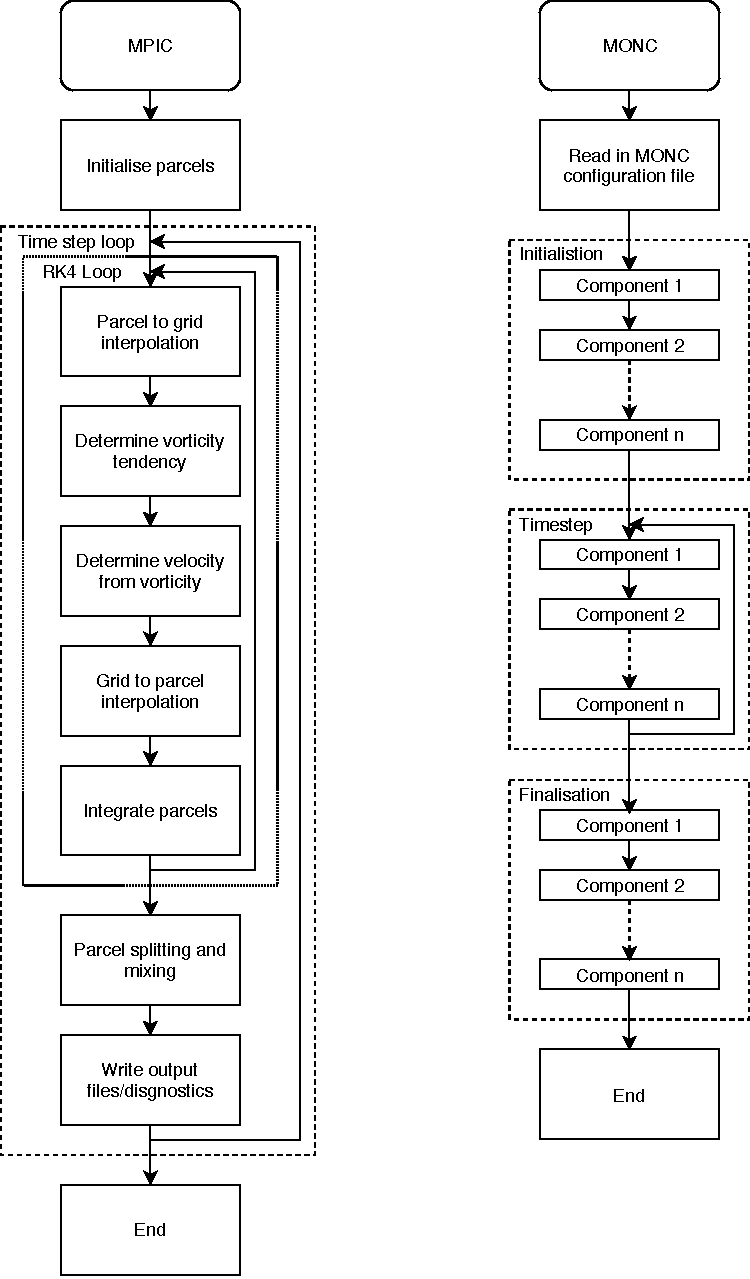
\includegraphics[scale=0.42]{pmpic_images/flowchart.pdf}
  \end{center}
\end{frame}

\section{Design and performance}

%-------------------------------------------------------------------
\begin{frame}
\frametitle{eCSE project}
\textit{A fully Lagrangian dynamical core for the Met Office NERC Cloud Model}
\vspace{0.2cm}
\begin{center}
St Andrews, Leeds, EPCC (Mich\`ele Weiland, Nick Brown, Gordon Gibb)
\end{center}

\vspace{0.1cm}
Ideas:
\begin{itemize}
\item Harness {\gr MONC's parallelism}: hybrid OpenMP+MPI.
\item Poisson solver available.
\item Approach: {\bl domain decomposition}, number of parcels per subdomain will vary (simplicity versus optimal load balancing).
\item {\re Lagrangian diagnostics} can feed back into standard MONC.
\item {\pu Component testing} using simplified code.
\end{itemize}

\end{frame}

\begin{frame}
\frametitle{Parallelism}

\vspace{0.2cm}
\begin{itemize}
\item Vector Poisson solver: requires global communication. {\bl Efficient algorithms} exist.
\item First implementation OpenMP. Inherent limitation of problem size. HPC trend to {\pu large distributed memory systems}. 
\item Much more {\re parcel data} than {\gr grid data}.
\item Parcel data: {\oran local communication}.
\end{itemize}

\centering

\end{frame}

\begin{frame}
\frametitle{PMPIC}
\begin{itemize}
\item Implementation of MPIC in MONC's framework.
\item Based on stripped version of MONC core.
\item Not compatible with other MONC components (parcels in model state, RK4 time step, different equations, non-staggered grid).
\item But uses (FFTs, grids) and extends (parcel parallelism) MONC infrastructure.
\item GIT repository + makefile.
\end{itemize}
\end{frame}


\begin{frame}
\frametitle{Design choices}
\begin{itemize}
\item Data held in arrays, rather than parcel-types (more difficult halo-swap, but efficient). \\
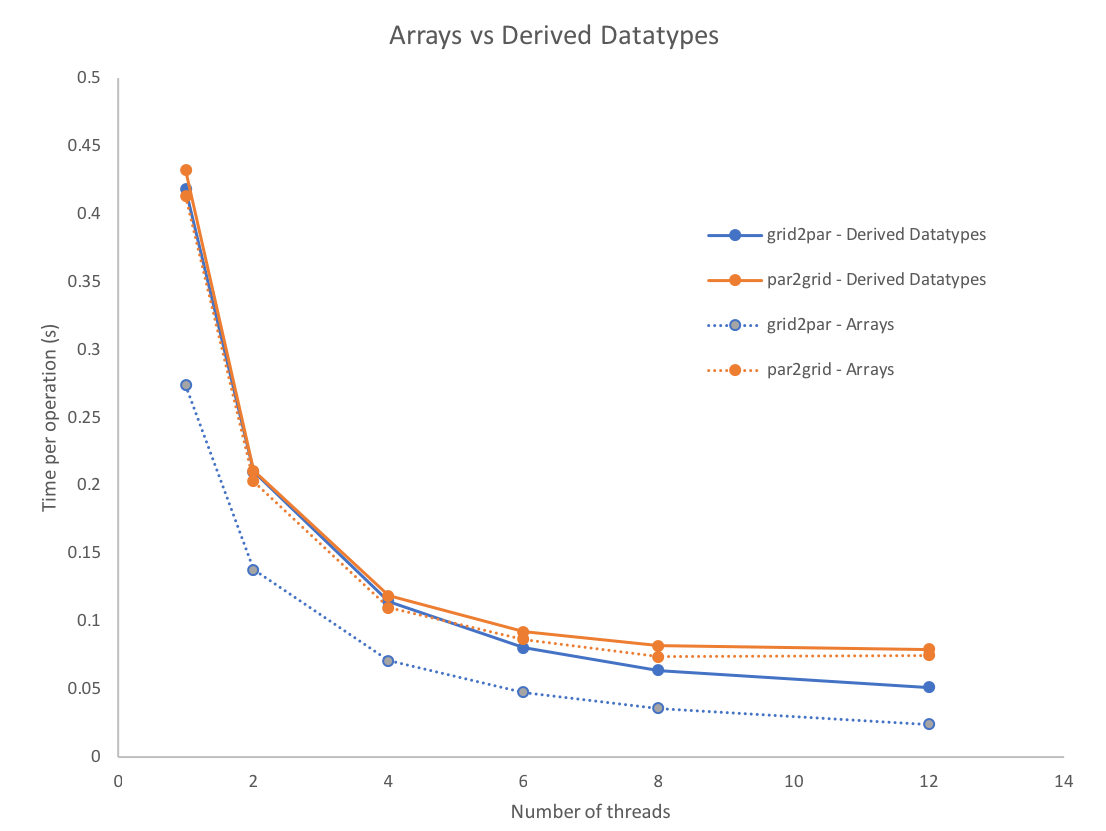
\includegraphics[width=0.45\textwidth]{pmpic_images/grid2par.png} 
\item New group type: RK4 (not all operations substepped). Note: higher memory footprint.
\item Binary dumps (parcels/grids) and NetCDF (optional, grids only so far), instead of IO-server. Memory requirements of main code.
\end{itemize}

\end{frame}

\begin{frame}
\frametitle{Halo-swapping}
\begin{itemize}
\item Parcel halo-swap needed testing. In particular: backfill.
\item Modified grid halo-swap in solver. Decision to write new simple halo-swapper for grids. 
\item Halo-swapping also comes into parcel mixing. Systematic parcel creation/removal tests.
\end{itemize}

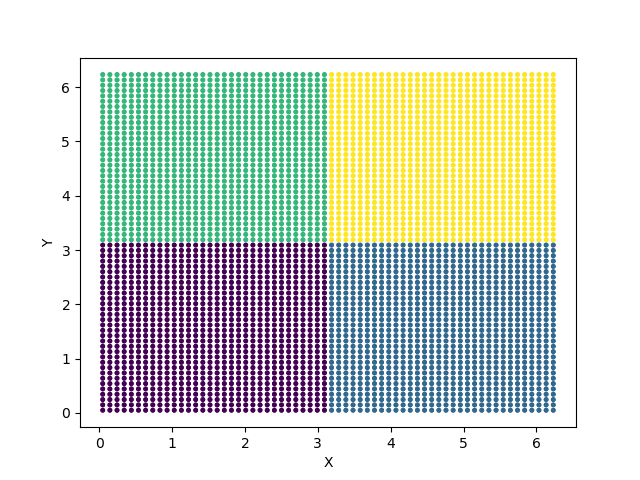
\includegraphics[width=0.45\textwidth]{pmpic_images/vel0.png} 
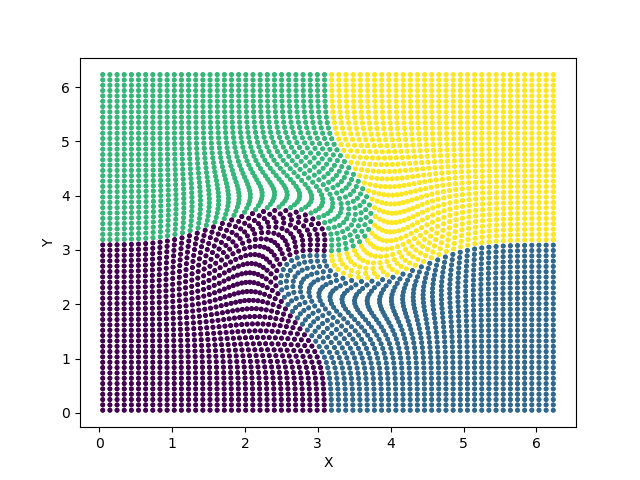
\includegraphics[width=0.45\textwidth]{pmpic_images/vel1.png} 

\end{frame}

\begin{frame}
\frametitle{Numerics}
\begin{itemize}
\item 4th order compact central differencing in tridiagonal solver (David Dritschel).
\end{itemize}

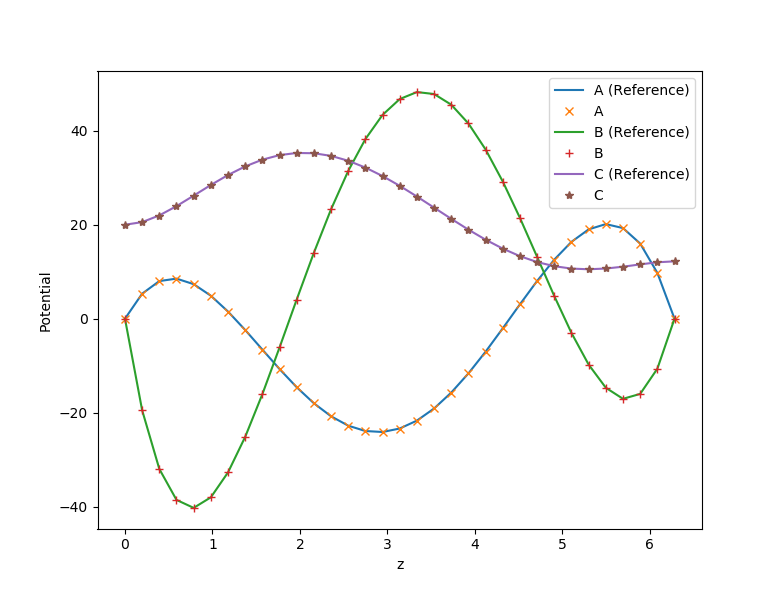
\includegraphics[width=0.70\textwidth]{pmpic_images/solution.png} 

\end{frame}

\begin{frame}
\frametitle{Performance: single node}

\begin{itemize}
\item Overall performance of new code on single core: 1.6 times faster.
\item MPI scaling hindred by load imbalance.
\item OpenMP not scaling well (tune chunk size/try static arrays?).
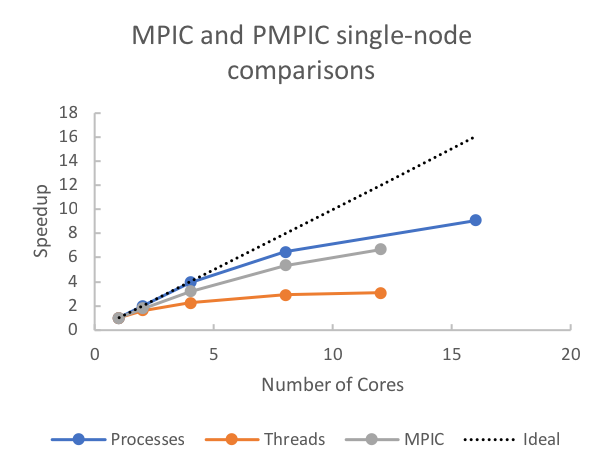
\includegraphics[width=0.45\textwidth]{pmpic_images/singleNode.png} 
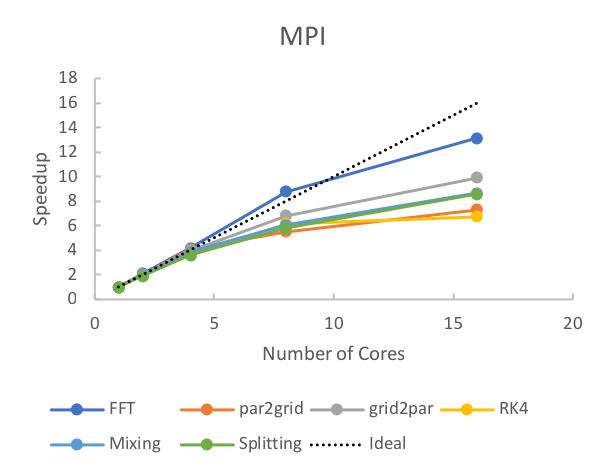
\includegraphics[width=0.45\textwidth]{pmpic_images/MPISingle.png} 
\end{itemize}

\end{frame}

\begin{frame}
\frametitle{Performance}

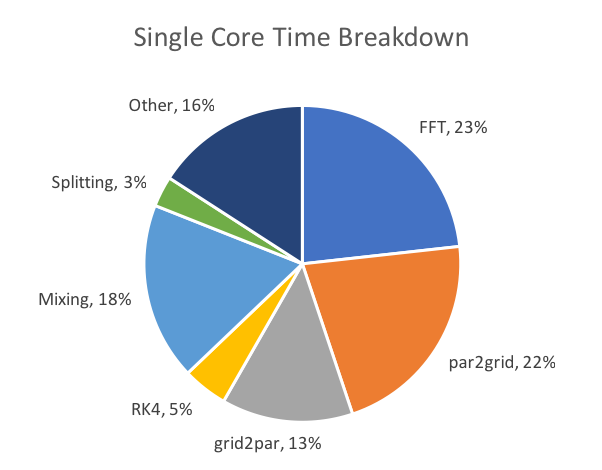
\includegraphics[width=0.90\textwidth]{pmpic_images/pie.png} 

\end{frame}

\begin{frame}
\frametitle{Performance: large simulations}

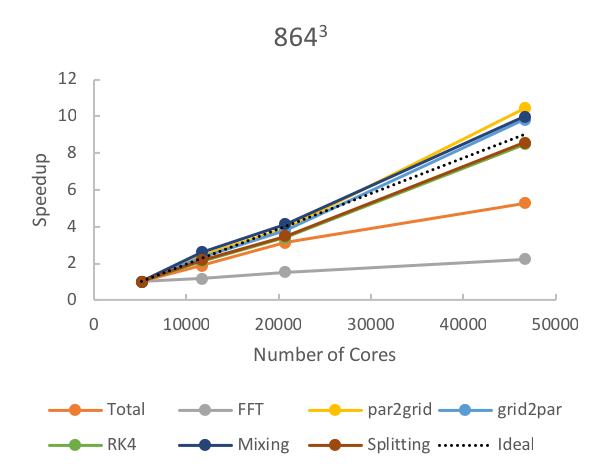
\includegraphics[width=0.45\textwidth]{pmpic_images/864.png} 
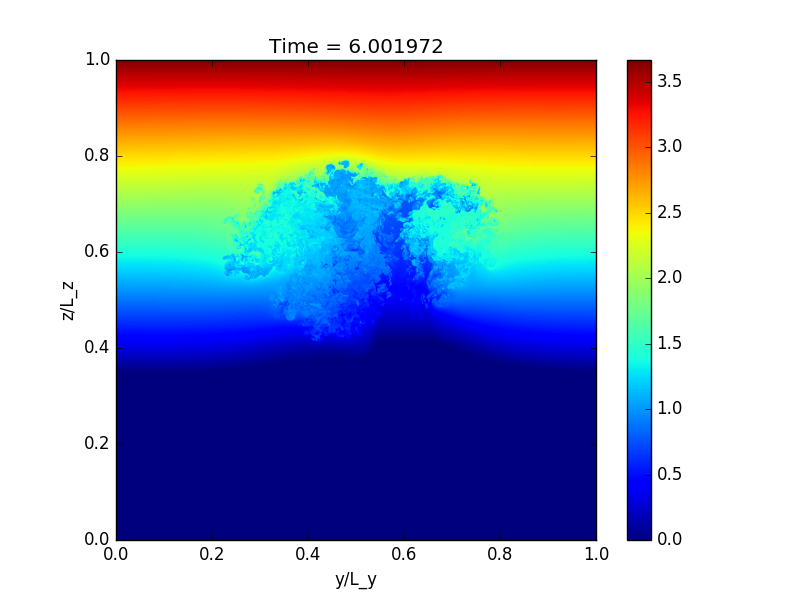
\includegraphics[width=0.45\textwidth]{pmpic_images/6.png} 

\end{frame}


\begin{frame}
\frametitle{Benefits}

\begin{itemize}
\item First use of this type of model in atmospheric community.
\item Massively parallel MPIC will make it more attractive for {\pu other problems}, e.g. ocean mixed layer, density-laden flows.
\item {\bl Alternative approach} for MONC community.
\item Could provide basis for Lagrangian diagnostics, currently {\re lacking in MONC}.
\item {\gr BSD} license.
\end{itemize}

\end{frame}

\hypertarget{welcome-to-the-pmpic-wiki}{%
\section{Repository, installation, adding components}\label{welcome-to-the-pmpic-wiki}}

\begin{frame}{PMPIC code repository}
\protect\hypertarget{pmpic-code-repository}{}

Example usage:

mpiexec -n 2 monc --config=config.mcf

Dependencies:

\begin{itemize}
\tightlist
\item
  MPI
\item
  FFTW
\item
  NetCDF (optional)
\end{itemize}

Compilers tested:

\begin{itemize}
\tightlist
\item
  GNU (on laptop and ARCHER)
\item
  Cray (on ARCHER)
\end{itemize}

\end{frame}

\begin{frame}
Default test case is a spherical moist and
warm thermal in a neutrally-stable boundary layer overlaid with a
stably-stratified atmosphere. 
\end{frame}

\begin{frame}[fragile]{Running PMPIC}
\protect\hypertarget{running-pmpic}{}

Running pmpic should be as simple as executing:

\texttt{{[}mpiexec/aprun\ ...{]}\ /path/to/monc\ -\/-config={[}config\ file{]}}

The config file controls which components are run (and in what order)
and also runtime parameters. There is also a global\_config file which
contains basic settings required for MONC to operate. This shouldn't be
edited unless you know what you're doing.

The config file and global\_config should be placed in the working
directory.

The final files should have timestep number 144, and using
\texttt{display\_parcels.py} as

\texttt{python\ display\ parcels.py\ 144\ {[}N{]}}

(where N is the number of processes used in the simulation).
%\includegraphics{https://user-images.githubusercontent.com/17198605/49156538-82419900-f315-11e8-89a3-8533f580acc8.png}

Congratulations you have successfully run PMPIC! The default case is small and should be able to run on a laptop in around a minute or less.

\end{frame}

\begin{frame}[fragile]{Further information}
\protect\hypertarget{further information}{}

When the code is slow, please first try running with

\begin{Shaded}
\begin{Highlighting}[]
\BuiltInTok{export} \VariableTok{OMP_NUM_THREADS=}\NormalTok{1}
\end{Highlighting}
\end{Shaded}

as by default OpenMP uses all cores on your system, so you may end out
running many more threads+processes than you have cores.

A list of components is provided on the PMPIC wiki

\end{frame}

\begin{frame}{Included scripts}
\protect\hypertarget{included-scripts}{}

display\_grid.py: displays a field (currently buoyancy)\\
display\_parcels.py: renders a field based on a Gaussian kernel\\
planner.py: calculates the approximate memory footprint of PMPIC (total
and per process)\\
timing.py: reads previously created timing data (need to specify this
beforehand in MONC configuration file)\\
visualise.py: older visualisation routine (obsolete?)

\end{frame}

\begin{frame}{Subgrid visualisation}

\begin{figure}
  \begin{center}
    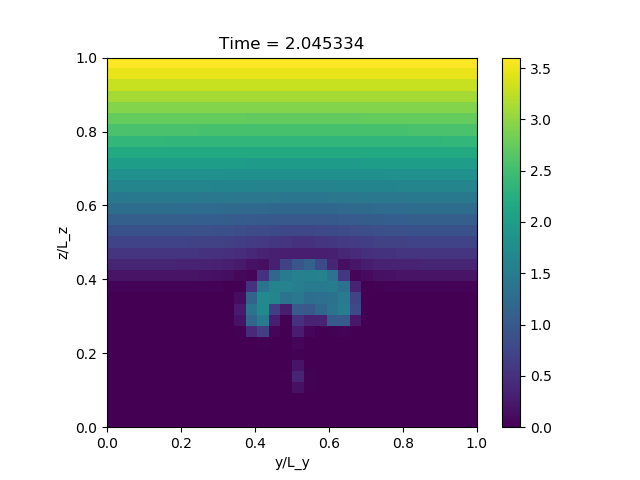
\includegraphics[scale=0.3]{pmpic_images/32grid.png}
    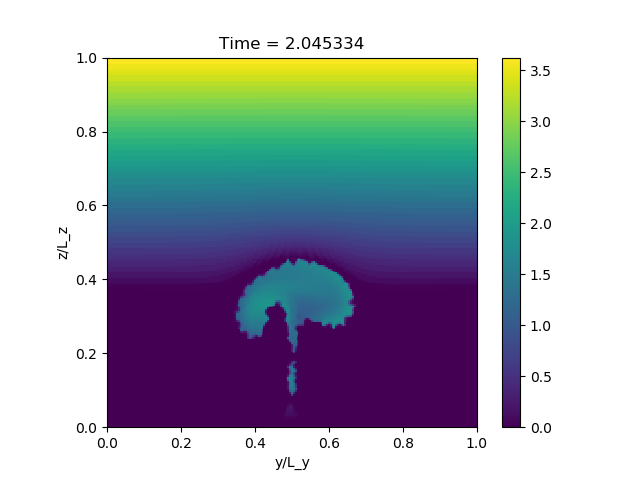
\includegraphics[scale=0.3]{pmpic_images/32parcels.png}
  \end{center}
  \caption{Comparison of the buoyancy in the $z-y$ plane for a $32^3$ grid cell simulation constructed from the gridded values (left) and from the parcels (right). It can be seen that images constructed from the parcels have considerably more detail as they are able to resolve sub-gridcell structure. \label{lowres}}
\end{figure}

\end{frame}

\begin{frame}[fragile]{Writing your own initial condition component}
\protect\hypertarget{writing-your-own-initial-condition-component}{}

PMPIC comes with two initial condition components
\begin{itemize}
\item \texttt{basic\_parcelsetup} component (which places parcels uniformly in
space but does not assign any values to them)
\item \texttt{plume\_parcelsetup} component which sets up the initial
condition used
\href{https://rmets.onlinelibrary.wiley.com/doi/10.1002/qj.3319}{here}.
\end{itemize}

To write your own initial condition component, it is easiest to create a
copy of the \texttt{basic\_parcelsetup} directory in
\texttt{components/} and call it something else (let's say
\texttt{my\_parcelsetup}). Change into this directory and alter the name
of \texttt{src/basic\_parcelsetup.F90} to
\texttt{src/my\_parcelsetup.F90}. Also remember to modify the makefile
in this directory to point to the newly renamed file.

Now to edit \texttt{my\_parcelsetup.F90}. First of all, change the
module name to \texttt{my\_parcelsetup\_mod}. Change the
\texttt{basic\_parcelsetup\_get\_descriptor} function to (next slide)
\end{frame}

\begin{frame}[fragile]

\begin{footnotesize}
\begin{Shaded}
\begin{Highlighting}[]
\DataTypeTok{type(component_descriptor_type)} \KeywordTok{function}\NormalTok{ my_parcelsetup_get_descriptor()}
\NormalTok{    my_parcelsetup_get_descriptor%name}\KeywordTok{=}\StringTok{"my_parcelsetup"}
\NormalTok{    my_parcelsetup_get_descriptor%version}\KeywordTok{=}\FloatTok{0.1}
\NormalTok{    my_parcelsetup_get_descriptor%initialisation}\KeywordTok{=}\OperatorTok{>}\NormalTok{initialisation_callback}

\KeywordTok{end function}\NormalTok{ my_parcelsetup_get_descriptor}
\end{Highlighting}
\end{Shaded}
\end{footnotesize}

Now you can go and edit the subroutine \texttt{initalisation\_callback}
to put in the initial conditions you want.

To enable this component, alter your config file to have the line
\texttt{my\_parcelsetup\_enabled=.true.} (ensuring that the other
parcelsetup components are disabled).

After recompiling monc you should now be able to use your new component!

\end{frame}

\begin{frame}[fragile]{NetCDF libraries}
\protect\hypertarget{netcdf-libraries}{}

We have made output to NetCDF available in PMPIC. This requires a
version of NetCDF with parallel NetCDF support

These libraries are available under ARCHER as the cray-hdf5-parallel and
cray-netcdf-hdf5parallel modules. Note that if you change compiler
environment (compilation has been tested with the GNU compiler on
ARCHER) you may need to unload and then reload the modules.

See PMPIC wiki for details on local compilation.

\end{frame}
 
\section{Conclusions and future work}

\begin{frame}
\frametitle{Conclusions}

\begin{itemize}
\item eCSE outcome: MPIC model that scales on thousands of cores.
\item Improving scalability: analyse issues with OpenMP, replace FFT-derivatives by compact finite differencing where possible (currently 18 FFTs per time step).  
\end{itemize}

\end{frame}

%-------------------------------------------------------------------

\begin{frame}
\frametitle{Future plans for MPIC}

\vspace{0.2cm}
\begin{itemize}
\item Realistic {\bl thermodynamics} and {\bl precipitation}. From idealised to atmospheric model.
\item More flexible {\pu boundary conditions}, in particular for momentum.
\item Work on {\re marginally resolved and subgrid-scale dynamics} to improve mixing representation (convergence).
\item Exploitation of {\oran vorticity diagnostics} and {\oran Lagrangian analysis}. 
\end{itemize}

\centering

\end{frame}

%%%%%%%%%%%%%%
\end{document} 
%%%%%%%%%%%%%%
